\chapter{Evaluation}
\label{chap:evaluation}
We will evaluate the success of this project by analysing the proportion of tasks the agent is able to successfully complete. We will compare these results to similar approaches in the field \cite{one-shot-imitation, one-shot-pose-estimate}.
As described in these papers, the methods used for one-shot imitation learning generalise well to completing the same tasks with different objects. For example picking up a different water bottle to the one in the demonstration. We also know that they generalise to different environment setups, robust to rotations and translations of the objects in the scene. We hope that this project will allow the agent to generalise even further beyond, to skills which differ conceptually to those shown in the demonstrations. We hope that this extra level of generalisability will provide improved success rate metrics on unseen tasks compared to the state of the art current solutions. The existing solutions appear to limit their unseen test set to the same categories of task as their training set, just with new unseen objects. We hope that in this project we can expand this test set to a much more wide spread of potential tasks, and still see high success rates in the testing phase.\\

In addition to evaluating our algorithm under ideal conditions we would like to investigate how robust it is to its starting configuration. Due to the design of the learning algorithm, it is likely that the ability to learn new skills will be affected by the quality of initial demonstrations. We hypothesise that an agent given 10 unique and diverse demonstrations, will perform better in unseen task completion, than an agent trained with 10 demonstrations which all just involve picking up similar objects. This is because the algorithm as proposed, learns through augmenting existing demonstrations with noise. As such, the skills the agent will learn are likely to conceptually branch off of an existing skill. If the initial skill set is very diverse, then this allows the agent to search a wider portion of the space of all trajectories. Comparatively, if the initial skills are all very similar, then the agent has a harder time searching wide in the search space since it can only save a new skill by augmenting existing skills. A simplified example of this is shown in Figure \ref{fig:trajectory-space} with a 2D search space. In practice the space of all trajectories is far more than 2 dimensions. This makes having diverse initial skills which cover the search space as best as possible even more important since there is far more for the agent to search.

\begin{figure}[ht]
    \centering
    \begin{subfigure}[b]{0.45\textwidth}
        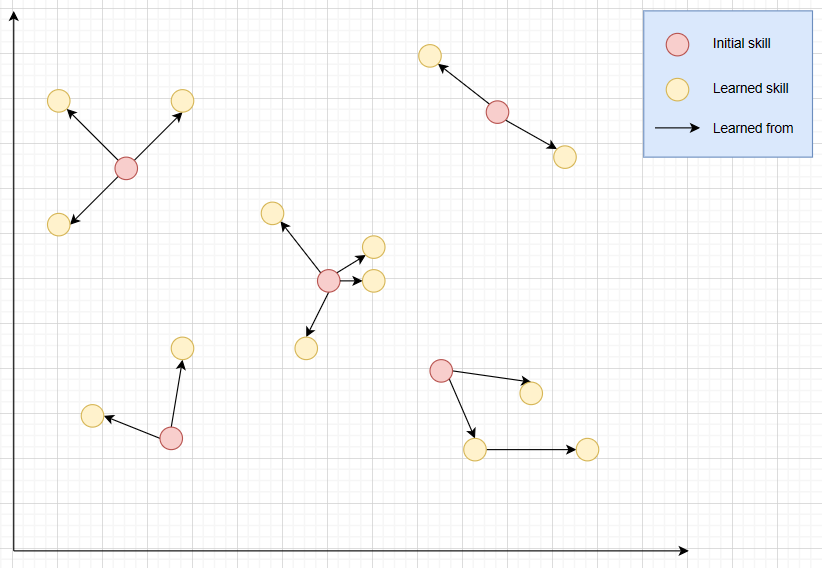
\includegraphics[width=\textwidth]{figures/graph_spread.PNG}
        \caption{Diverse initial skill set}
    \end{subfigure}
    \hfill
    \begin{subfigure}[b]{0.45\textwidth}
        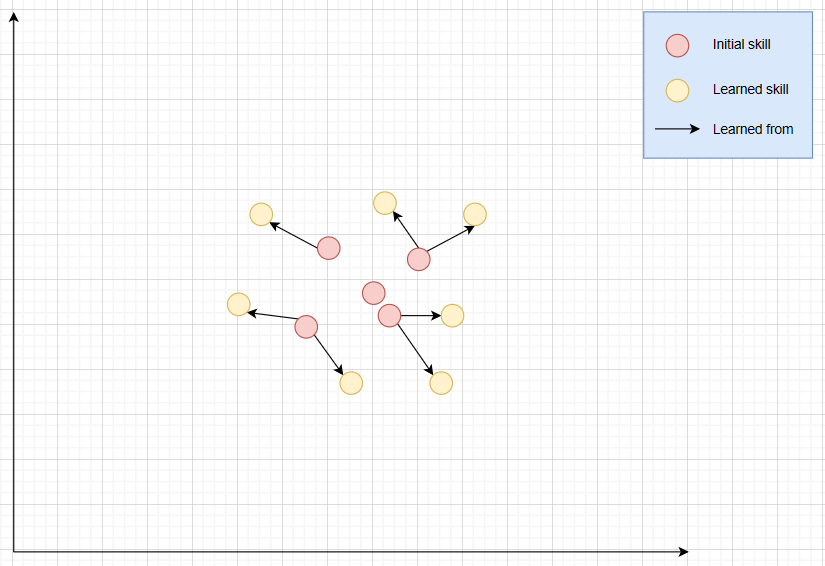
\includegraphics[width=\textwidth]{figures/graph_narrow.PNG}
        \caption{Narrow initial skill set.}
    \end{subfigure}
    \caption{Simplified diagram of trajectory search space.}
    \label{fig:trajectory-space}
\end{figure}

In Figure \ref{fig:trajectory-space} nodes of the graph represent the trajectories which succeed in performing some task and are saved as a skill. Edges represent that the child skill was learned by augmenting the parent skill. Nodes with no parent are the initial skill set, coloured red.